\section{Device}

In this section we describe the physical implementation of the bandpass filter including details of how the chosen circuit parameters were realized on the physical chip.

\subsection{Layout}

A micrograph of the device is shown in Fig.\,\ref{Fig:deviceMicrograph}.
The device has four qubit-resonator pairs all coupled in parallel to a common filter.
The filter is implemented as a $\lambda/4$ coplanar waveguide resonator embedded into the feed line.
The feed line is interrupted on one side with a capacitor forming a voltage antinode, and is shorted to ground on the other side forming a voltage node.
The resulting standing wave mode is used as the filter resonance.
The measurement resonators are coupled capacitively in parallel to a single common filter, and each measurement resonator is capacitively coupled to a qubit.

\begin{figure}
\begin{centering}
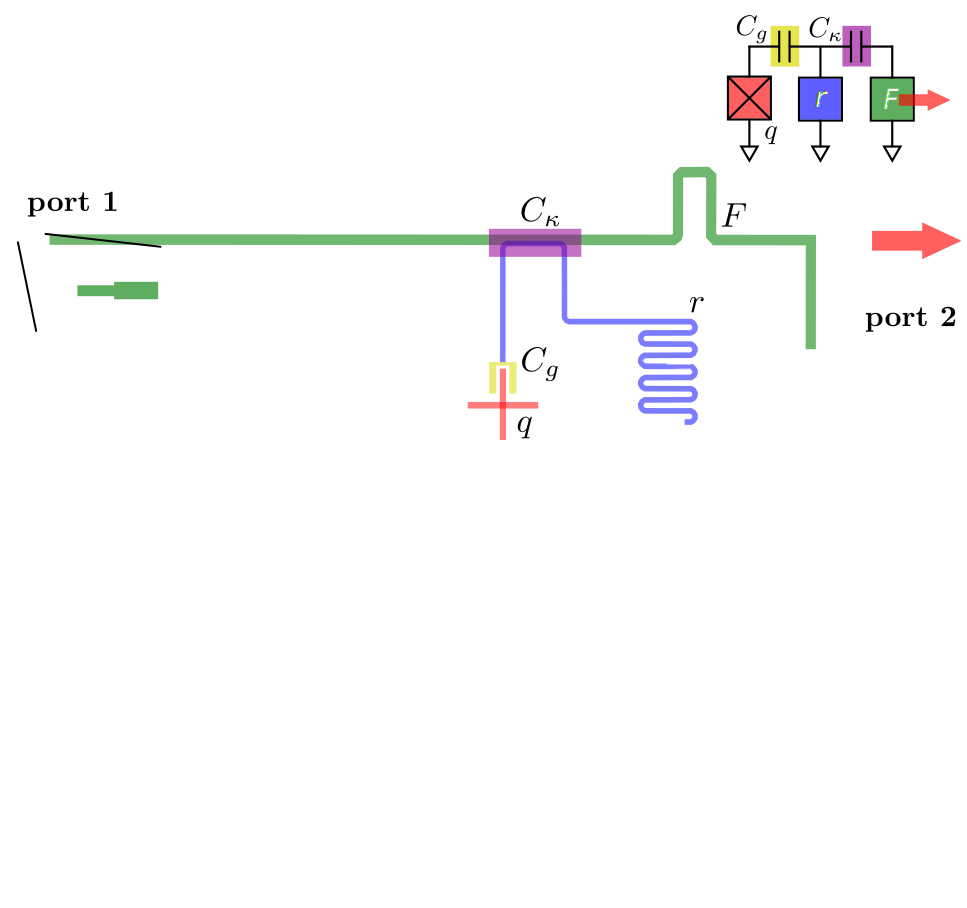
\includegraphics[width=\textwidth]{deviceMicrograph.pdf}
\par\end{centering}
\caption{Micrograph of the device. The false color corresponds to the colors used in the lumped element model, shown in the top right inset. Signals enter the system through a feed line at port 1. The filter $F$ is formed by a standing wave resonator embedded into the feed line. The feed line is interrupted by a capacitance (left inset) at one end and shorted to ground on the other, forming a $\lambda/4$ resonance. Signals injected at port 1 are mostly reflected by the weak input capacitance. The transmitted energy rings up the filter resonance. Energy leaves the filter through a tap near the shorted end at port 2. The red arrow indicates the path by which energy leaves the filter through a wire bond (not shown) and enters the external detection hardware, including a parametric and HEMT amplifier. The measurement resonators $r$ are connected to the filter via capacitance $C_{\kappa}$ formed by the proximity of the filter and resonator traces. The resonator couples to the qubit $q$ through an inter-digitated capacitor $C_g$. Note that the design allows for an independent resonator for each qubit while allowing several resonators to share a single filter. Note also the filter requires near zero additional on-chip area.}
\label{Fig:deviceMicrograph}
\end{figure}

\subsection{Filter}

The filter is implemented as a $\lambda/4$ coplanar waveguide resonator.
The voltage node is formed by connecting the waveguide to ground.
The voltage antinode is formed at signal input point (port 1 in Fig.\,\ref{Fig:deviceMicrograph}) where the filter connects to the feed line through a capacitor.

\subsubsection{Length}

The length of the filter is related to the desired frequency by \begin{equation}
l = \frac{\lambda}{4} = \frac{\pi v}{2 \omega_F} = \frac{\pi c}{2 \omega_F \sqrt{\epsilon_{\text{eff}}}} \end{equation}
where $c$ is the speed of light in vacuum and $\epsilon_{\text{eff}}$ is the relative relative dielectric constant of the waveguide.
For a coplanar waveguide with trace and gap widths much smaller than the thickness of the substrate, we have $\epsilon_{\text{eff}} = (1 + \epsilon_s) / 2$ where $\epsilon_s$ is the relative dielectric constant of the substrate.
In our experiment we used sapphire substrate with $\epsilon_s = 10.4$ giving $\epsilon_{\text{eff}} = 5.7$.
For a filter frequency of $\omega_F/2\pi = 6.75\,\text{GHz}$ this gives $l = 4,654\,\mu\text{m}$.

\subsubsection{Input capacitance}

The value of the input capacitance $C_{\text{in}}$ is determined by the amount by which we allow the input line to load the filter.
The loaded quality factor $Q_l$ of a resonant mode of frequency $\omega_0$ and self capacitance $C$ connected to a resistor environment $R_e$ through a coupling capacitor $C_c$ is \begin{equation}
Q_l = \frac{C}{\omega_0 R_e C_c^2}. \end{equation}
For the filter we rename the parameters $\omega_0 \rightarrow \omega_F$, $C_c \rightarrow C_{\text{in}}$, and $Q_l \rightarrow Q_{\text{in}}$. Using the effective capacitance of our $\lambda/4$ filter resonator $C = \pi / 4 \omega_F Z_0$, assuming that $R_e=Z_0$, and solving for $C_{\text{in}}$ gives \begin{equation}
C_{\text{in}} = \sqrt{\frac{\pi}{4 \omega_F^2 Z_0^2 Q_{\text{in}}}}. \end{equation}
In our device we used $\omega_F / 2\pi = 6.75\,\text{GHz}$, $Q_{\text{in}} = 40 \times Q_F = 1200$, and $Z_0 = 50 \Omega$, which gives $C_{\text{in}} = 12 \, \text{fF}$.

This capacitance was implemented as a parallel plate SiO$_2$ dielectric capacitor, as shown in Fig.\,\ref{Fig:filterInputCapacitance}\,a.
The dielectric thickness was $t = 200\,\text{nm}$.
With the relative permittivity of SiO$_2$ of 3.9, this required a plate area of $A = C t / 3.9 \epsilon_0 = 70 \, \mu m ^2$, which is a modest and readily achievable size.
Most importantly, this small size avoids the problem of large ground plane cuts which would be needed if we were to implement $C_{\text{in}}$ as an interdigitated capacitor.

The SiO$_2$ has a relatively large loss tangent, making it unsuitable for use in the qubit or measurement resonator.
With $\tan\delta \approx 3\times 10^{-4}$, and corresponding $Q_{\text{SiO}_2} \approx 3,000$ \cite{OConnell:microwaveLoss2008}, a resonance using SiO$_2$ dielectric capacitors would have $T_1 \approx 80\,\text{ns}$ at 6\,GHz.
However, this is not an issue for the filter.
The output circuitry strongly loads the filter, in our case giving $Q_F \sim 30$.
With $Q_F \ll Q_{\text{SiO}_2}$ the dissipation from the dielectric is much smaller than the photon loss rate through the output circuit.
Therefore, the SiO$_2$ in the filter's input capacitor contributes a negligible fraction of the total loss presented to the qubit, and absorbs a negligible fraction of the dispersed measurement photons.

\subsubsection{Input capacitor electrical length}

Because of the finite impedance of the input capacitor, the voltage antinode point is not actually a true $\lambda/4$ distance from the voltage node.
In other words, the capacitor adds electrical length to the waveguide.
This effect must be counterbalanced by modifying the waveguide's geometric length.
To compute the necessary adjustment we treat the capacitor as an effective length of transmission line by writing \begin{equation}
\phi_c = 2 \omega_F d_c / v \end{equation}
where $d_c$ is the effective length of the capacitor, $v$ is the propagation speed in the waveguide, and $\phi_c$ is the phase shift incurred by reflection from the capacitor.
See Fig.\,\ref{Fig:filterInputCapacitance}\,b for an illustration.
The phase shift is computed as \cite{Pozar:microwaveEngineering2009} \begin{equation}
\phi_c = \angle \left( \frac{Z_L - Z_0}{Z_L + Z_0} \right) \end{equation}
where $Z_L = 1/i\omega C_{\text{in}} + Z_0$ is the series impedance of the capacitor and feed line loading the filter resonance, and $Z_0$ is the characteristic impedance of the line (we assume the filter and feed line characteristic impedances are equal).
Combining these results yields \begin{equation}
d_c = \frac{c}{2 \omega_F \sqrt{\epsilon_{\text{eff}}}} \angle \, \left( \frac{Z_L - Z_0}{Z_L + Z_0} \right) \label{eq:C_inElectricalLength} \end{equation}
which is the length by which the geometric length of the line must be reduced to maintain a resonance frequency of $\omega_F$.

Using this and the previously chosen value $C_{\text{in}}=12\,\text{fF}$ we compute the effective length of the capacitor to be $d_c = 75\,\mu m$.
This length must be subtracted from the geometric length of the filter coplanar waveguide.

\begin{figure}
\begin{centering}
\includegraphics[width=0.6\textwidth]{filterInputCap.pdf}
\par\end{centering}
\caption{Input capacitor for the filter. a) Micrograph of the device. The feed line comes in from the left and the filter coplanar waveguide resonator is on the right. A thin film of SiO$_2$ separates the connecting aluminum strip on the feed line side. A hole in the feed line renders the overlap area insensitive to optical lithography misalignment. The connecting strip contacts the filter resonator directly. b) Circuit model. A wave reflecting from the input capacitor acquires a phase shift which effectively increases the length of the filter.}
\label{Fig:filterInputCapacitance}
\end{figure}

\subsubsection{Output tap point - $Q_F$}

The dispersed signals exits the filter through a tap off wire connected to the filter near its voltage node.
The position of the tap determines the rate at which energy leaves the filter, thus setting $Q_F$, as we now explain.
The voltage profile of the resonant mode in the distributed resonator has a cosine shape $V \propto \sin \left( \pi x/ 2 l \right)$ where $x=0$ is the voltage node at the shorted end and $x=l$ is the voltage antinode at the open end.
If the tap were placed at $x=0$ where the voltage is zero it would carry no energy away from the filter and the coupling $Q$ induced by the tap would be infinity.
If the tap were placed at the voltage antinode at $x=l$ it would feel the maximum of the filter voltage and would be accurately modeled as a shunt resistor in a lumped element equivalent circuit of the filter.
Placing the tap at a distance $x$ from the voltage node reduces the power dissipated by $R_e$ by a factor of the square of the relative voltage, $\sin \left( \pi x / 2 l \right)^2$, yielding \begin{equation}
Q_F = \left. Q_F \right|_{x=l} / \sin \left( \pi x / 2 l \right)^2. \label{eq:Q_FVsTapPosition} \end{equation}
where $\left. Q_F \right| _{x=l}$ is the quality factor we would compute from a lumped element model.

In the lumped element model the loaded $Q$ is given simply by $\left. Q_F \right|_{x=l} = R_e / Z_F^0$ where $R_e$ is the resistance of the circuit external to the tap, $Z_F^0 = 4Z_0/\pi$ is the characteristic impedance of the filter mode, and $Z_0$ is the filter transmission line characteristic impedance.
Combining this with Eq.\,(\ref{eq:Q_FVsTapPosition}) in the case $R_e = Z_0$ gives \begin{equation}
Q_F = \frac{\pi / 4}{\sin \left( \pi x / 2 l \right)^2} \approx \frac{(l/x)^2}{\pi}. \end{equation}
We designed for $Q_F=30$ to get a filter bandwidth of $\sim\,200\,\text{MHz}$, giving $x = 0.1 \times l$.

\subsubsection{Bond pad inductance}

Proper flow of return currents is essential to the design of the filter resonator.
In Figure \ref{Fig:bondPadInductance} we show the shorted end of the filter with the tap off through which the signal leaves the filter and enters an amplification chain.
Part of the current return path is interrupted by the wire bond pad as shown in the figure.
The large perimeter of the bond pad would introduce inductance into the return path and shift the frequency of the filter resonance.
To correct this we used SiO$_2$ dielectric crossovers to tie the ground planes on either side of the tap off path together, thus shorting the inductance presented by the bond pad.

\subsubsection{Summary}

Here we summarize the steps in the design of the filter:
\begin{enumerate}
 \item From the desired frequency $\omega_F$ compute the geometric length according to \begin{displaymath}
 l = \pi c / (2 \omega_F \sqrt{\epsilon_{\text{eff}}}). \end{displaymath}
 \item Choose a loaded quality factor $Q_F$ to get the desired filter bandwidth $\Delta \omega_F$, according to $Q_F = \omega_F / \Delta \omega_F$.
 \item Choose an input capacitance $C_{\text{in}}$ by requiring that the loading from the input $Q_{\text{in}}$ is much ($100\times$) larger than $Q_F$. The capacitance is determined by \begin{displaymath}
 C_{\text{in}} = \sqrt{\frac{\pi}{4 \omega_F^2 Z_0^2 Q_{\text{in}}}} \end{displaymath}
 \item Compute the electrical length of the input capacitor according to \begin{displaymath}
 d_c = \frac{c}{2\omega_F \sqrt{\epsilon_{\text{eff}}}} \angle \left( \frac{Z_L - Z_0}{Z_L + Z_0} \right) \end{displaymath}
 and adjust the geometric length by this amount.
 \item Choose the output tap point $x$ according to \begin{displaymath}
 Q_F = \frac{\pi / 4}{\cos \left( \pi x / 2 l \right)^2} \end{displaymath}
 and ensure that crossovers are used to connect the ground planes on either side of the tap.
\end{enumerate}

\begin{figure}
\begin{centering}
\includegraphics[width=0.5\textwidth]{bondPadInductance.pdf}
\par\end{centering}
\caption{Micrograph of the filter tap off point and bond pad. Without crossovers, part of the current return path would flow around the wire bond pad, as shown by the dotted line. The large perimeter of the bond pad would introduce inductance into the return path of filter current and shift the frequency of the filter. Dielectric crossovers connect the ground planes on either side of the tap off path, thus shorting the inductance of the bond pad.}
\label{Fig:bondPadInductance}
\end{figure}

\subsection{Measurement resonators}

The measurement resonators, like the filter, were implemented as $\lambda/4$ coplanar waveguide resonators.
In this section we explain how we designed the coupling between the measurement resonators and qubits, and between the measurement resonators and the filter.

\subsubsection{Qubit-resonator coupling: claw coupler}

The resonators were capacitively coupled to the qubits.
Dielectric parallel plate capacitors like the one used for the filter input capacitor could not be used, as the loss tangent of SiO$_2$ of $\sim 3\times10^{-4}$ \cite{OConnell:microwaveLoss2008}, would limit the qubit $T_1$.
Instead, we used interdigitated capacitors as shown in Fig.\,\ref{Fig:clawCoupler}, which we have nicknamed the ``claw''.
The claw not only couples the resonator to the qubit, but also forms a large capacitance to ground.
This capacitance to ground changes the resonator's effective length similarly to the filter input capacitor, although the effect is somewhat more complex as the claw also adds significant geometric length.

With no reliable means to analytically compute the effect, we instead used the Sonnet\footnote{www.sonnetsoftware.com} numerical electromagnetic simulation package to find the phase shift incurred by reflection from the claw.
The coupling capacitance $C_g$ between the qubit and resonator, and the phase incurred by reflection from the claw was found as a function of frequency and claw length $L$.
The results of the simulation were fit with second order polynomial curves as given in Tables \ref{Table:CgToL} and \ref{Table:LToPhi}.

Here we summarize the design of the claw couplers:
\begin{enumerate}
 \item From the desired coupling strength $g$ the value of $C_g$ is chosen from Eq.\,(\ref{eq:C_gVsg}).
 \item Use the data from Table \ref{Table:CgToL} to find the appropriate length $L$ of the claw.
 \item Use the data from Table \ref{Table:LToPhi} to find the phase shift imposed by the claw. This phase is then converted to an effective length in the same way as was done for the filter.
 \item Adjust the resonator length to account for the phase shift.
\end{enumerate}

\subsubsection{Resonator-filter coupling: parallel line coupler}

The capacitive coupling between the measurement resonators and filter was implemented by allowing their center traces to run parallel over a length $w$ to allow in-plane, as shown in Fig.\,\ref{Fig:resonator-filterCoupling}.
The measurement resonator and filter traces are separated by a strip of ground plane of width $x$ to keep the ground plane equipotential.
The parameters $x$ and $w$ were adjusted to get the desired coupling capacitance $C_{\kappa}$.
This capacitance was computed numerically using Sonnet in a procedure entirely similar to that described above for the resonator-qubit coupling.
The results of the Sonnet simulation are summarized in Table\,\ref{Table:couplerArm}.

The coupling capacitance $C_{\kappa}$ was determined by the desired ring-up rate of the resonator $\kappa_r$.
From Eq.\,(\ref{eq:Q_r}) we find \begin{equation}
\kappa_r = \left( \frac{4}{\pi} \right)^2 \omega_r^3 Q_F Z_0^2 C_{\kappa}^2 \longrightarrow C_{\kappa} = \frac{\pi}{4} \sqrt{\frac{\kappa_r}{Q_F Z_0^2 \omega_r^3}}\end{equation}
where we've used $Q_r = \omega_r / \kappa_r$. For $\kappa_r^{-1} = 50\,\text{ns}$ and $Q_F=30$ we find $C_{\kappa} = 1.47\,\text{fF}$.

\begin{table} \begin{center} \begin{tabular}{  c  c  c  c  }
\hline \hline
Frequency [GHz]	&	\quad	$p_0$	&	\quad $p_1$	&	\quad	$p_2$ \\
\hline
4.8 & -0.7610256 & 23.42786129 & -30.03751643 \\
5.0 & -0.75985036 & 23.40431259 & -30.03256152 \\
6.705 & -0.74027938 & 23.11730508 & -29.92148358 \\
6.735 & -0.73999725 & 23.11213134 & -29.91986705 \\
6.765 & -0.73971394 & 23.10693518 & -29.91824295 \\
6.805 & -0.73933434 & 23.09997203 & -29.91606597 \\
\hline \hline
\end{tabular}
\end{center}
\caption{Claw length $L$ as a function of qubit-resonator coupling capacitance $C_g$. For each frequency, the claw length and capacitance are related according to $L/\mu\text{m} = \sum_{n=0}^2 p_n (C_g/\text{fF})^n $.}
\label{Table:CgToL}
\end{table}

\begin{table} \begin{center} \begin{tabular}{  c  c  c  c  }
\hline \hline
Frequency [GHz]	&	\quad	$p_0$	&	\quad $p_1$	&	\quad	$p_2$ \\
\hline
4.8 & 1.52E-007 & -1.24E-003 & -8.51E-002 \\
5.0 & 1.61E-007 & -1.29E-003 & -8.87E-002 \\
6.705 & 2.47E-007 & -1.74E-003 & -1.19E-001 \\
6.735 & 2.49E-007 & -1.74E-003 & -1.19E-001 \\
6.765 & 2.50E-007 & -1.75E-003 & -1.20E-001 \\
6.805 & 2.53E-007 & -1.76E-003 & -1.21E-001 \\
\hline \hline
\end{tabular}
\end{center}
\caption{Phase shift $\phi$ as a function of claw length $L$. For each frequency the phase shift and claw length are related by $\phi / \text{rad} = \sum_{n=0}^2 p_n (L/\mu\text{m})^n$.}
\label{Table:LToPhi}
\end{table}

\begin{table} \begin{center} \begin{tabular}{  c  c  c  c  }
\hline \hline
x [$\mu\text{m}$]	&	\quad	$p_0$	&	\quad $p_1$	&	\quad	$p_2$ \\
\hline
2 & 0.00367265 & 64.6536 & -53.9095 \\
5 & 0.0169587 & 101.302 & -61.7247 \\
8 & 0.0382334 & 143.915 & -68.7105 \\
\hline \hline
\end{tabular}
\end{center}
\caption{Coupling arm length $w$ as a function of capacitance $C_{\kappa}$ for several values of the width $x$ of the ground plane strip. For each value of $x$, $w$ is related to $C_{\kappa}$ according to $w/\mu\text{m} = \sum_{n=0}^2 p_n (C_{\kappa}/\text{fF})^n$.}
\label{Table:couplerArm}
\end{table}

\begin{figure}
\begin{centering}
\includegraphics[width=0.5\textwidth]{clawCoupler.pdf}
\par\end{centering}
\caption{The interdigitated capacitor connecting the measurement resonator and qubit. Note the thin wire connecting the ground plane on either side of the topmost qubit finger. This wire is an ``in-plane crossover'' connecting together the ground plane on either side of the qubit finger.}
\label{Fig:clawCoupler}
\end{figure}

\begin{figure}
\begin{centering}
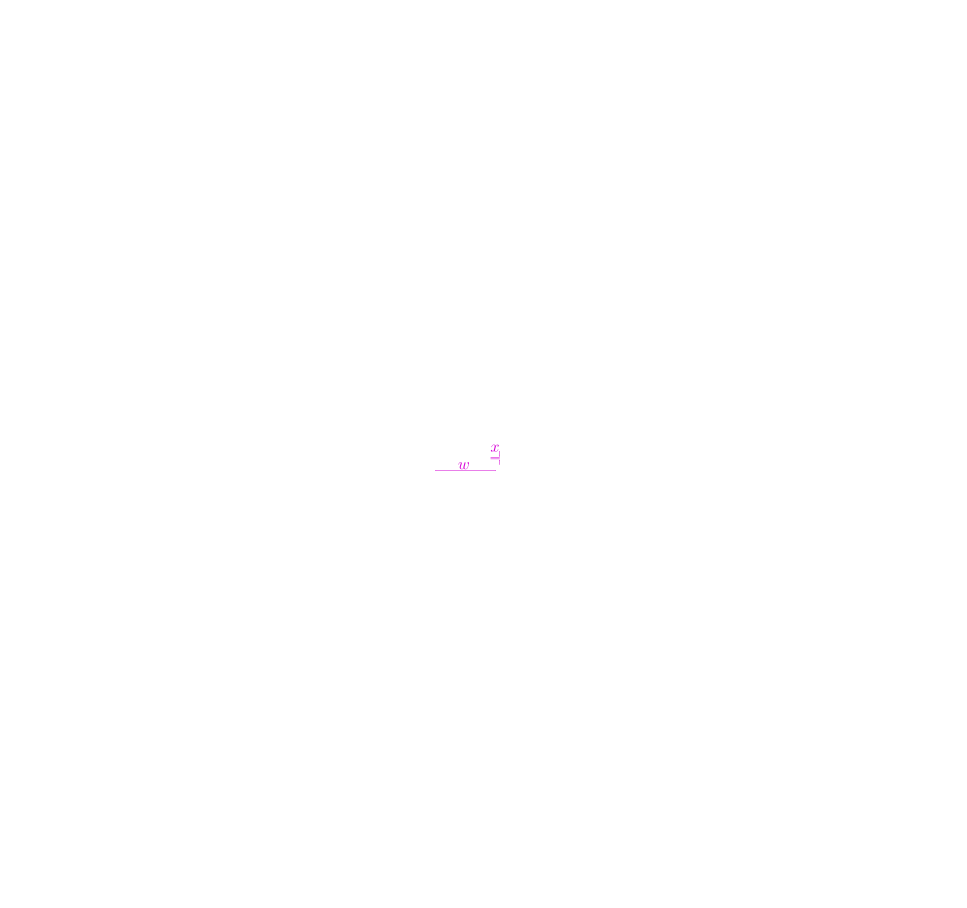
\includegraphics[width=0.8\textwidth]{resonator-filterCoupling.pdf}
\par\end{centering}
\caption{Coupling between a measurement resonator and the filter.}
\label{Fig:resonator-filterCoupling}
\end{figure}


\subsection{Mode shape coupling factor}

Because the voltage profile in a distributed resonator is not constant, the capacitances coupling the measurement resonators required a position dependent adjustment.
Each capacitance was multiplied by \begin{displaymath}
\left[ \cos \left(\pi x_r / 2 l_r \right) \cos \left(\pi x_F / 2 l_F \right) \right]^{-1} \end{displaymath}
where $x_r$ is the distance of the coupler from the measurement resonator voltage antinode, and $x_F$ is the distance of the coupler from the filter voltage antinode.


\subsection{Parameters}

Using the results contained in Tables \ref{Table:CgToL}, \ref{Table:LToPhi}, and \ref{Table:couplerArm} we converted the values of $C_g$ and $C_{\kappa}$ from Table \ref{Table:circuitParameters} to physical dimensions for use in the fabricated device.


\section{Fabrication}

The device was made of thin film aluminum film deposited on a sapphire substrate. Silicon dioxide was used as a dielectric layer for the filter input capacitor and for wiring crossovers used to connect the ground planes. The Josephson junctions were made of an Al/AlO$_x$/Al tri-layer. The fabrication process is summarized in the following steps:
\begin{enumerate}
 \item{Defined control lines and resonators.}
 \begin{enumerate}
  \item{Approximately 100\,nm of aluminum is deposited on a 3 inch sapphire wafer via electron beam evaporation in a Plassys evaporator.}
  \item{A pattern defining the measurement resonators, filter, input/output lines, and qubit control lines is etched into the film using using optical lithography and chemical etching in an inductively coupled plasma (ICP) etcher with BCl$_3$/Cl$_2$.}
 \end{enumerate} 
 \item{Dielectric crossovers are formed to bridge the ground planes on either side of the measurement input and output lines, and the qubit control lines.}
 \begin{enumerate}
  \item{A 200\,nm thick layer of silicon dioxide is deposited through an optically defined photoresist mask to form the insulating layer of the crossovers in a lift-off procedure.}
  \item{A photoresist mask defining the crossover wires is defined through optical lithography. The sample is placed in the Plassys chamber and the underlying aluminum film is ion milled \emph{in situ} to remove the native oxide layer. A new aluminum layer is deposited through a photoresist mask to form the crossover wires via lift-off.}
 \end{enumerate}
 \item{The cross shape of the transmon qubit is etched into the base aluminum layer via the same method used to define the control lines and resonators. This step is done apart from the control lines and resonators so that the qubit features are subjected to a lower number of subsequent processing steps. This separation of etch steps for the control lines and resonators from the etch step for the qubit has not definitely been shown to improve qubit coherence. It was done as a cautionary measure.}
 \item{An alignment mark pattern, to be used in the next step, is formed with electron beam evaporated gold via lift-off.}
 \item{The Josephson junctions are formed using double angle shadow mask evaporation in the Plassys chamber. The shadow mask is formed via electron beam lithography. This step uses the previously defined gold alignment marks to align the electron beam pattern with the optical patterns from previous steps. The base layer is ion milled \emph{in situ} prior to the junction deposition to remove the native oxide.}
\end{enumerate}